\begin{figure}[H]
  \centering
  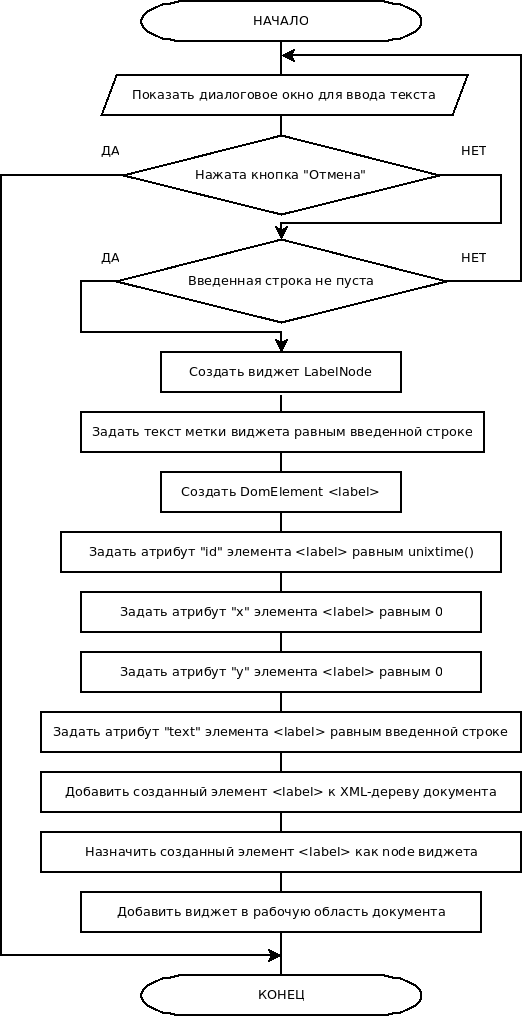
\includegraphics[width=0.55\textwidth]{diagrams/block-schemes/add-label.png}
  \caption{Алгоритм добавления метки в схему}
  \label{fig:new-label}
\end{figure}

Как видно из рисунка \ref{fig:new-label}, процесс добавления метки в документ сопровождается, во-первых, созданием виджета с текстом и, во-вторых, добавлением нового узла в XML-дерево документа.

\begin{figure}[H]
  \centering
  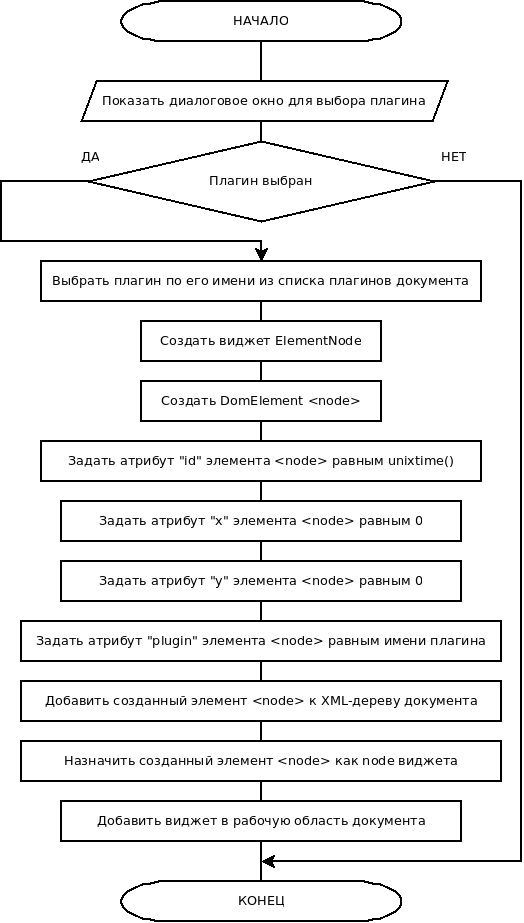
\includegraphics[width=0.6\textwidth]{diagrams/block-schemes/add-node.png}
  \caption{Алгоритм добавления узла в схему}
  \label{fig:new-node}
\end{figure}

Добавление узла, как показано на рисунке \ref{fig:new-node}, протекает аналогичным с описанным на рисунке \ref{fig:new-label} способом.

\begin{figure}[H]
  \centering
  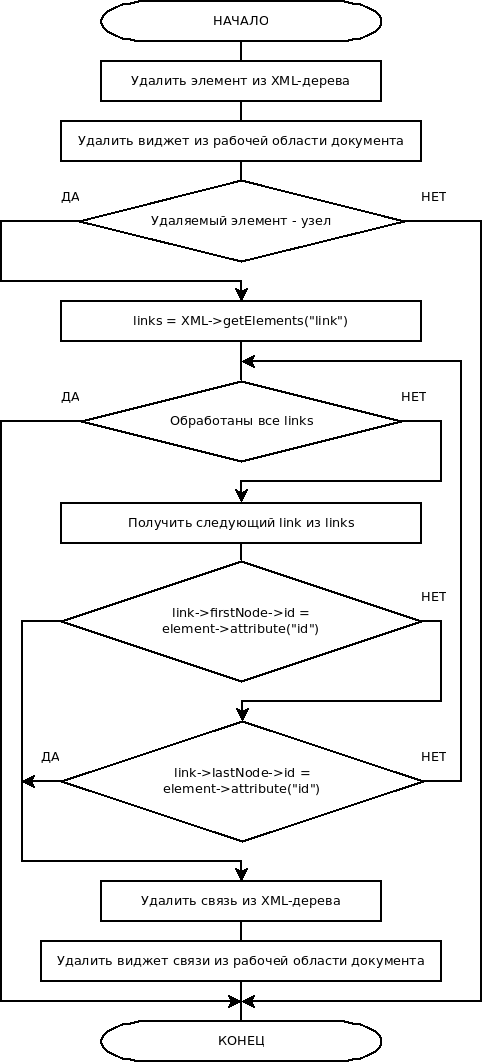
\includegraphics[width=0.55\textwidth]{diagrams/block-schemes/delete.png}
  \caption{Алгоритм удаления элемента из схемы}
  \label{fig:delete-node}
\end{figure}

Из рисунка \ref{fig:delete-node} видно, что удаление узла ведет к удалению соединенных связей.

\begin{figure}[H]
  \centering
  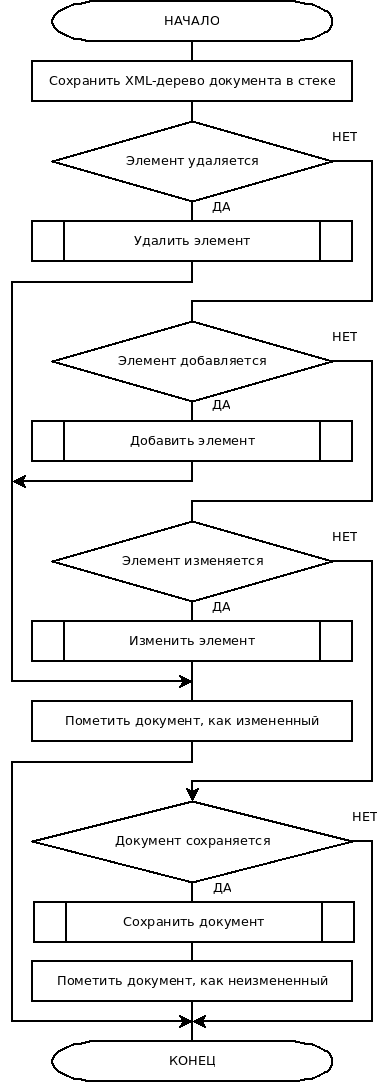
\includegraphics[width=0.45\textwidth]{diagrams/block-schemes/change.png}
  \caption{Обобщенный алгоритм работы с документом}
  \label{fig:change}
\end{figure}

На рисунке \ref{fig:change} показано, что любые изменения документа влекут смену признака состояния на <<изменен>>.
При сохранении документа указанный признак сбрасывается.

\begin{figure}[H]
  \centering
  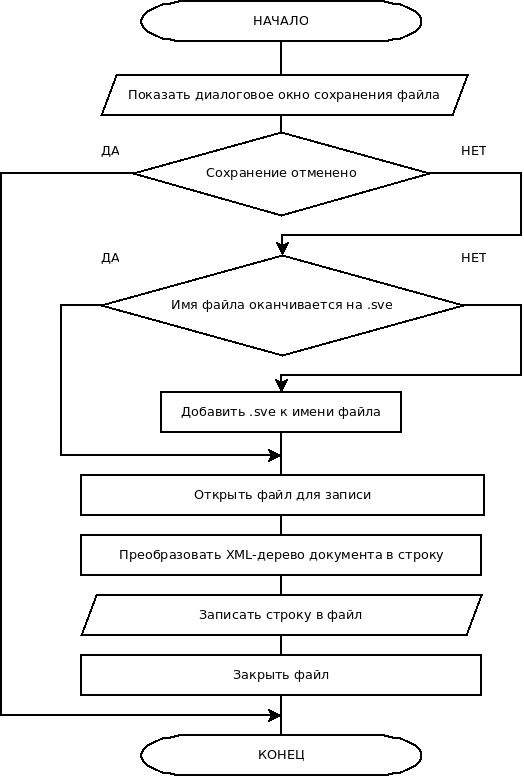
\includegraphics[width=0.6\textwidth]{diagrams/block-schemes/save.png}
  \caption{Алгоритм сохранения документа}
  \label{fig:save-file}
\end{figure}

Сохранение документа, как видно из рисунка \ref{fig:save-file}, заключается в переносе содержимого XML-дерева документа в текстовое представление и записи его на диск.

\begin{figure}[H]
  \centering
  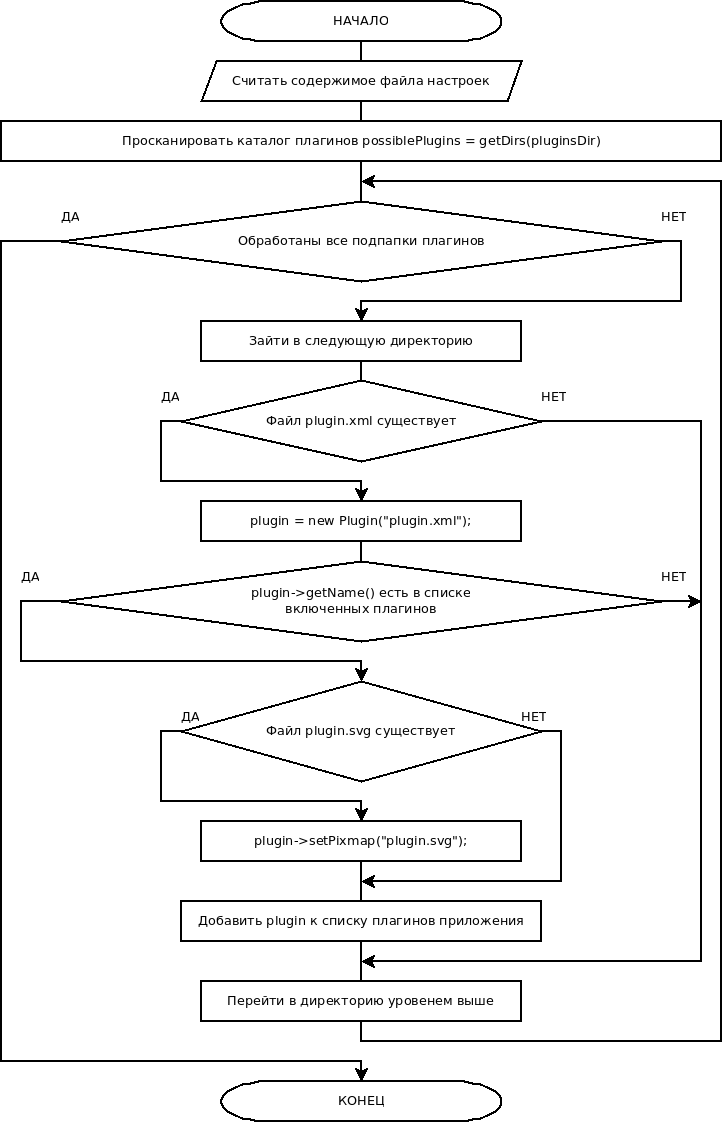
\includegraphics[width=0.77\textwidth]{diagrams/block-schemes/start.png}
  \caption{Алгоритм запуска программы}
  \label{fig:start}
\end{figure}

При запуске, как показано на рисунке \ref{fig:start}, просматриваются все папки внутри директории расширений в поисках файлов расширений.
Необходимость подключения определяется по наличию расширения среди включенных в настройках.

\begin{figure}[H]
  \centering
  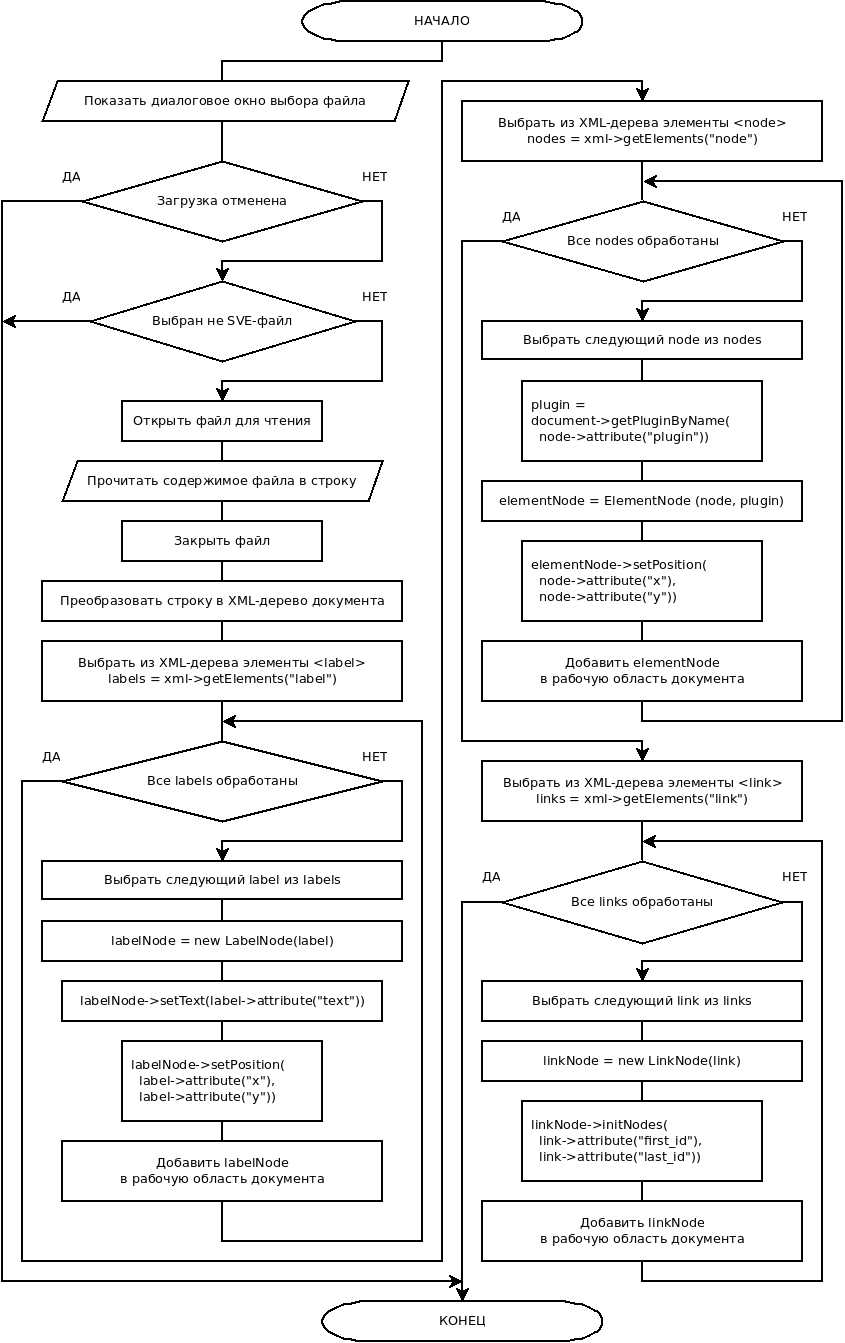
\includegraphics[width=0.87\textwidth]{diagrams/block-schemes/load.png}
  \caption{Алгоритм загрузки документа}
  \label{fig:load-file}
\end{figure}

Загрузка документа, как видно из рисунка \ref{fig:load-file}, протекает в два этапа: перенос содержимого файла в XML-дерево документа и создание на основе данного дерева виджетов в рабочей области.

\begin{figure}[H]
  \centering
  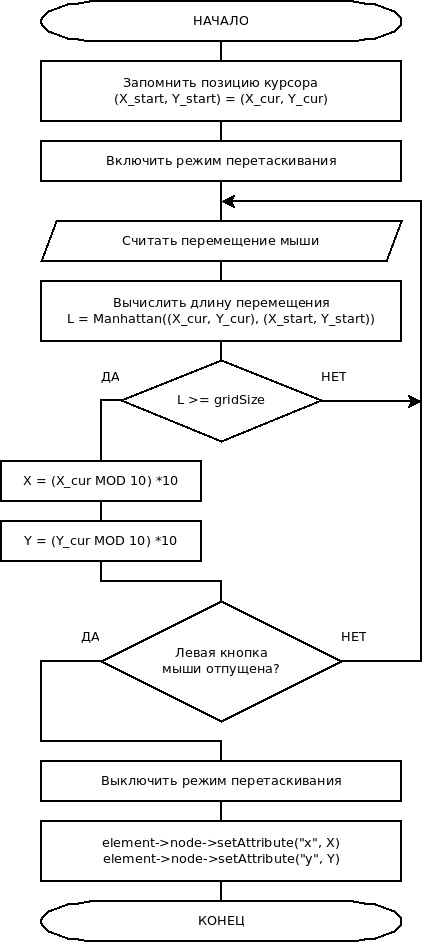
\includegraphics[width=0.48\textwidth]{diagrams/block-schemes/drag.png}
  \caption{Алгоритм перетаскивания элемента}
  \label{fig:drag}
\end{figure}

На рисунке \ref{fig:drag} показано, что элементы в схеме перетаскиваются по сетке с шагом в 10 пикселей.